\documentclass{ximera}

\title{How is my work scored?}

\begin{document}
\begin{abstract}
  We explain how your work is scored.
\end{abstract}
\maketitle

We want you to learn from this text. Hence, we ask questions to
``push'' your thinking, and leave blanks in examples to ensure you are
following along. We encourage you to \textbf{keep a notebook} where
you write each question and your answers, along with each major
theorem and example. In essence we want you to imagine that \textbf{we
  are writing mathematics together}, and thus are exploring a new
world of mathematics together.

With this in mind, your work is graded on the basis of its correct
\textbf{completion}. The green bar above
\begin{image}
  
\includegraphics{partialBar.png}
\end{image}
tells you how close you are to completion. We hope that you can
complete each activity and see a full green bar:
\begin{image}
  
\includegraphics{fullGreen.png}
\end{image}
However, sometimes there is a bug that prohibits a ``full green bar.''
In that case, do not despair, as we take these bugs into account when
grading. Moreover, please \textbf{let us know} any issues you are
having. If possible \textbf{we will fix the issue}.

If a correction is made then we may make an update. In this case an orange button will appear at the top of the screen:
\begin{image}
  
\includegraphics{update.png}
\end{image}
If you click the ``update'' button, a dialog will appear:
\begin{image}
  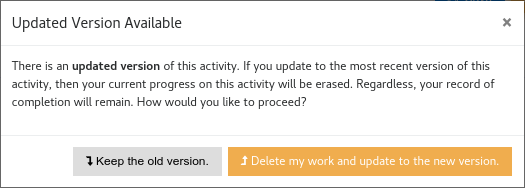
\includegraphics{updateDialog.png}
\end{image}
If you update your work, the current activity will be replaced by a
new activity. Since your previous work was for the previous
incarnation of the activity, your previous work will be
deleted. However, if you've completed the activity, \textbf{your
  record of completion remains}. You can witness this by selecting
another activity, and observing your green-bar for the updated
activity.  Unfortunately, if your activity was not complete before you
updated and you want a full green-bar on the updated activity, you
will have to complete the activity again.


We simply want you to learn and to provide you with the best possible
learning experience.

\begin{problem}
  Are you ready to start doing some math!?!
  \begin{multipleChoice}
    \choice[correct]{Yes I am!}
  \end{multipleChoice}
  \begin{hint}
    We promise the real course will not be this corny.
  \end{hint}
\end{problem}


\end{document}
